\section{Antarctic boundary recovery and conditional hindcasts}

\subsection{Recovered initial state and alternative forcing}
The initial Antarctic state is specified more fully than the first assessment
recognized. Shaffer's hindcasts begin at 240 kyr before CE 2000 with radius
$1.8636\times 10^6$ m and convert $24.78\times 10^{15}$ m$^3$ to 57 m of sea-level
equivalent\cite{shaffer}. We now integrate this initial-value problem using
independent proxy and instrumental inputs. NOAA Dome C and Spratt records use
years before 1950; they are converted to calendar years before comparison with
the model's different age origin. The W17F calibration dates of 118000,18000
and 4000 BCE correspond to 120,20 and 6 kyr before CE 2000\cite{wong2017fast}.

Antarctic air temperature combines Dome C anomalies, the global land--ocean
Mann EIV reconstruction, and HadCRUT4. We retain Shaffer's $-0.1$ K Dome C
adjustment, independently rebase Mann to 1961--1990, and apply the documented
modern amplification factor 1.2 around $-18^{\circ}$C. The independently
recomputed 500--1500 CE overlap adjustment would instead be $-0.168$ K;
the reconstruction variant and datum therefore remain explicit uncertainties.
The main alternative sea-level boundary subtracts Spratt's youngest 8.49 m
value and connects its CE 950 point to the first available Church--White annual
value at 1880.5. This interpolation is a declared assumption, not the recovered
Lambeck splice. An unshifted Spratt case and both archived Waelbroeck
chronologies test boundary sensitivity. These are observational proxy products,
not recycled DAIS hindcasts\cite{jouzel2007,spratt2016,mann2008,churchwhite2011,waelbroeck2002}.

The original transient subsurface-ocean history remains unrecovered. Shaffer's
written steady-state approximation supplies a useful alternative:
\begin{equation}
 T_o=0.00690T_a^2+0.439T_a+6.39\quad[^{\circ}\mathrm C].
\end{equation}
Here $T_a$ is Antarctic air temperature reduced to sea level. Applying this
formula during a transient omits ocean thermal memory. It permits a test of
the other equations without claiming recovery of the original DCESS forcing.

\subsection{Volume integration and switching dynamics}
The implementation advances physical ice volume by accumulation plus marine
discharge and independently inverts the verified geometric relation to obtain
radius at each integration stage. A separate radius-coordinate integration,
including the prescribed sea-level derivative, agrees with the volume solution.
All forcing knots and temperature gates split the integration grid; endpoint
stages use the branch valid within that interval.

The additional fast-loss flux follows the recovered temperature threshold and
stops below $18\times 10^{15}$ m$^3$\cite{wong2017fast}. Its cutoff creates a
discontinuous differential equation. When slow accumulation would increase
volume at the cutoff but full fast loss would decrease it, the mathematical
sliding solution holds volume at the cutoff by balancing those fluxes. Slow
mass loss can still lower volume below the cutoff. This continuation is
derived and tested on exact piecewise trajectories; it is not an assertion
about the original authors' timestep convention. Nineteen checks cover the
geometry inversion, coordinate equivalence, constant forcing, hitting times,
sliding and departure from the boundary.

For the central fixed-parameter hindcast, reducing the maximum step from 10 to 5
years changes saved sea-level equivalent by less than $8\times 10^{-8}$ m.
That numerical agreement does not remove the physical mismatch: the predicted
Last Interglacial contribution is $-0.17$ m, outside the written 3.6--7.4 m
window. Figure\ref{fig:paleo} compares input histories and their effects on this
result. It also tests initialization and the sharply different responses
obtained by changing the fast-loss threshold.

\begin{figure}[htbp]
\centering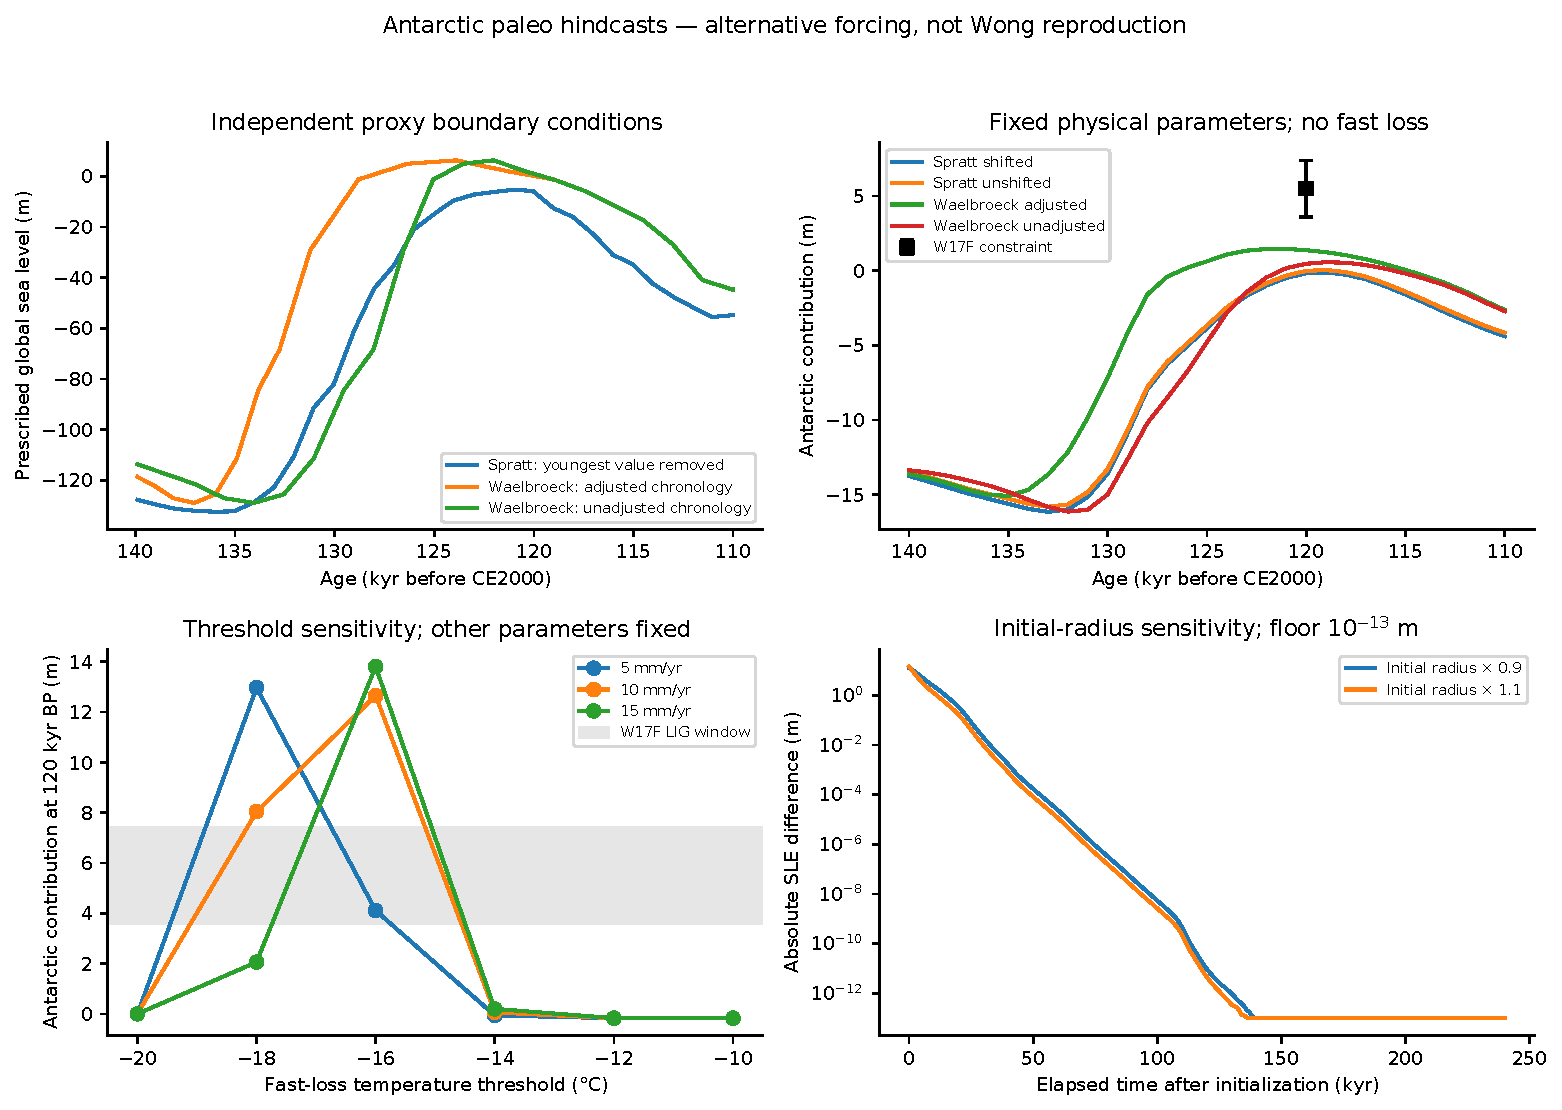
\includegraphics[width=\linewidth]{figures/dais_paleo_alternative.pdf}
\caption{Antarctic hindcasts under explicit alternative forcing. Upper left:
independent sea-level proxy inputs on a common calendar. Upper right:
fixed Shaffer case 4 parameters without fast loss, with the W17F Last
Interglacial constraint shown at 120 kyr before CE 2000. Lower left: fast-loss
rate and threshold sensitivities with other parameters fixed. Lower right:
differences after changing initial radius by 10\%; the plotting floor denotes
roundoff, not persistent physical differences. All panels are non-reproductions
of Wong's calibrated Antarctic ensemble.}\label{fig:paleo}
\end{figure}

\subsection{Conditional fitting and withheld annual rates}
A separate experiment varies discharge exponent $\gamma$, ocean partition
$\alpha$, fast-loss rate $\lambda$ and threshold $T_c$ over their documented
uniform ranges, fixing the remaining Shaffer parameters. Independent Latin
hypercube draws assess parameter coverage before a bounded coordinate search
minimizes the four standardized squared window residuals. The Last Interglacial
hard range is also checked. This restricted point fit omits additional
residual-process variance, uncertain forcing and the target joint calibration;
it is neither a posterior nor an independent test of those four fitted values.

Annual IMBIE mass-loss observations after 2002 provide a separate conditional
check. Observed temperatures remain prescribed in these years, and the
calibration's modern cumulative constraint ends in 2002. Figure\ref{fig:paleofit}
reports both parameter coverage and the later annual-rate errors. A good fit
to four widely separated volume constraints need not predict short-period
mass-loss variability.

\begin{figure}[htbp]
\centering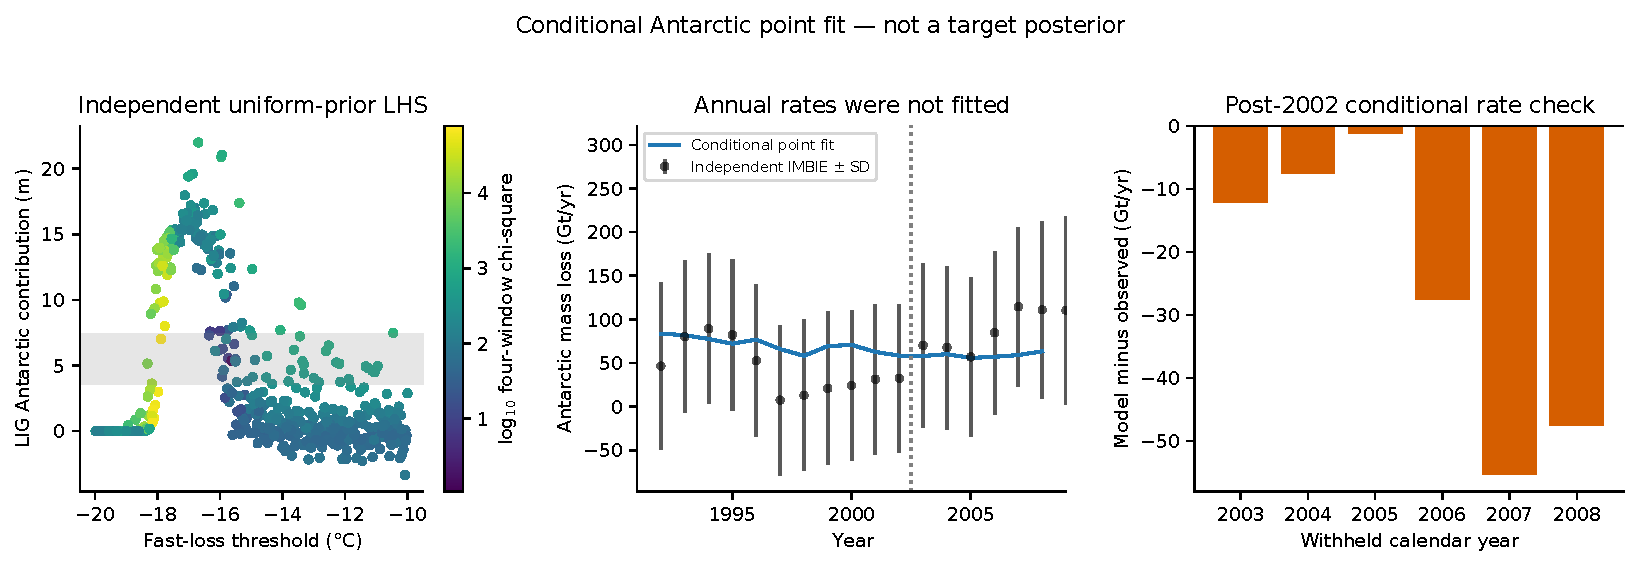
\includegraphics[width=\linewidth]{figures/dais_conditional_alternative.pdf}
\caption{Conditional Antarctic fitting under alternative forcing. Left:
independent uniform-prior Latin hypercube draws, coloured by four-window
misfit; shading marks the Last Interglacial range. Centre: fitted-model annual
mass loss and independent IMBIE observations with reported uncertainty. Right:
model minus observed rates after the 2002 cumulative constraint. No posterior
interval or recovered Wong result is implied.}\label{fig:paleofit}
\end{figure}
\begin{table}[htbp]
\centering\small
\begin{tabular}{lrrr}
\toprule
Constraint & Written mean (m) & Written SD (m) & Point fit (m) \\
\midrule
Last Interglacial & 5.5 & 0.95 & 5.5 \\
Last Glacial Maximum & -11.35 & 2.23 & -11.392 \\
Mid-Holocene & -2.63 & 0.68 & -2.7276 \\
1992--2002 increase & 0.00197 & 0.00046 & 0.001951 \\
\bottomrule\end{tabular}
\caption{Conditional Antarctic predictions under the explicitly alternative forcing. These four quantities are fitted, not held-out validation. The Last Interglacial hard acceptance interval is 3.6--7.4 m.}
\end{table}
The conditional solution uses $\gamma=1.93747$, $\alpha=0.02077$, $\lambda=0.01161$ m yr$^{-1}$ and $T_c=-15.62980\,{}^\circ$C. The search begins with 512 Latin hypercube points; 1 draws satisfy all four windows before local optimization. The final four-window $\chi^2$ is 0.02267. Halving the maximum timestep from 10 to 5 years changes these predictions by at most 2.7e-09 m. The conditional 2003--2008 mass-loss RMSE is 32.35 Gt yr$^{-1}$, with bias -25.22 Gt yr$^{-1}$. The observed and predicted mean rates are 84.17 and 58.96 Gt yr$^{-1}$, respectively.


The earlier64-point pilot reaches a different solution, with fast-loss rate
$0.015$ m yr$^{-1}$ and threshold$-15.484\,{}^\circ$C, while its four-window
$\chi^2=0.02354$ is almost unchanged. The larger search gives a lower misfit
without reaching that rate bound. These two fits illustrate conditional
parameter ambiguity; neither is presented as a uniquely inferred fast-loss
mechanism.

BRICK's written shore coupling is also recoverable: the Antarctic contribution
has fingerprint$-1$, while the other contributions have factor$+1$\cite{brick}.
Consequently, if $S_o$ is the sum of other components and $S_A$ is Antarctic
global sea-level change, the local boundary changes as $S_o-S_A$. A volume
integrator applies this feedback through geometric inversion at each stage.
An independent radius-coordinate calculation includes its derivative in
$\dot S$; ten checks cover that equivalence, equilibrium, timestep refinement
and component accounting. A lagged-input alternative follows the documented
previous-year forcing convention, while retaining an explicitly independent
within-year numerical integrator.
